\documentclass[aspectratio=169,urlcolor=black]{beamer}
\usetheme[language=ngerman,
titlepagelogo=logopolito,
bullet=circle,
pageofpages=of,
color=blue,
titleline=true
]{TorinoTh}

%\usepackage[ngerman]{babel}
%\usepackage[utf8]{inputenc}
\usepackage{tabularx}
\usepackage{booktabs}
\usepackage{multicol}
\usepackage{ulem}
\usepackage{makecell}
\usepackage{upgreek}
\usepackage{movie15}
%\usepackage{xcolor}
%\usepackage{isodate}
\hypersetup{colorlinks,linkcolor=black,urlcolor=black}
\addto{\captionsngerman}{%
  \renewcommand*{\contentsname}{Contents}
  \renewcommand*{\listfigurename}{Figures}
  \renewcommand*{\listtablename}{Tables}
  \renewcommand*{\figurename}{Fig.}	
  \renewcommand*{\tablename}{Tab.}
}
\newcommand*\mean[1]{\bar{#1}}
\newcommand{\tabitem}{~~\llap{\textbullet}~~}
\newcommand\widebar[1]{\mathop{\overline{#1}}}
\usepackage{caption}
\captionsetup{font=scriptsize}

\usepackage{color}
\usepackage{graphicx}
\usepackage{fancybox}
\usepackage[singlespacing]{setspace}

\usepackage{beamerthemesplit}
\usetheme[compress]{Heidelberg}
\definecolor{unirot}{rgb}{0.4,0.4,0.3} % babyblue 0,0.58,1
\usecolortheme[named=unirot]{structure}
%\setbeamercolor{alerted text}{fg=red}
\newcommand*\hilite[1]{\textcolor{red}{#1}}
%\def\hilite<#1>{%
  %\temporal<#1>{\color{black}}{\color{unirot}}%
               %{\color{gray}}}

\title[Light Transport Techniques for Tensor Field Visualization]{Light Transport Techniques for Tensor Field Visualization}
\subtitle{Master's Thesis Presentation}
\vspace*{2pt}
\author[Sebastian Bek]{Sebastian Bek\vspace*{7pt}}
\date{July 24th 2019}
\institute[Uni HD]{
Heidelberg University\\
Visual Computing Group (VCG)\\
Supervisors: Prof. Filip Sadlo, Dr. Susanne Krömker\\
}

%\color{unirot}{sebibek@gmail.com}
%\newsubfloat{figure}
\newcommand{\source}[1]{\hspace{-3pt} {\tiny \raisebox{-0.75in}{\rotatebox[origin=t]{90}{Source: \color{black}{#1}}}}}
\setlength{\belowcaptionskip}{-10pt}
\setlength{\intextsep}{-20pt}

\setlength{\skip\footins}{0.1cm}
\setlength{\footnotesep}{0.1cm}
\renewcommand\thempfootnote{\arabic{mpfootnote}}
\begin{document}

\frame[plain]{\titlepage}

\frame{
\frametitle{{Evaluation - Light Transport Gradient - Gyre Field}}
\begin{figure}[!t]
\centering
\caption*{\textit{Gyre test field}}\bigskip
  \begin{minipage}[t]{0.3\textwidth}
    \centering
  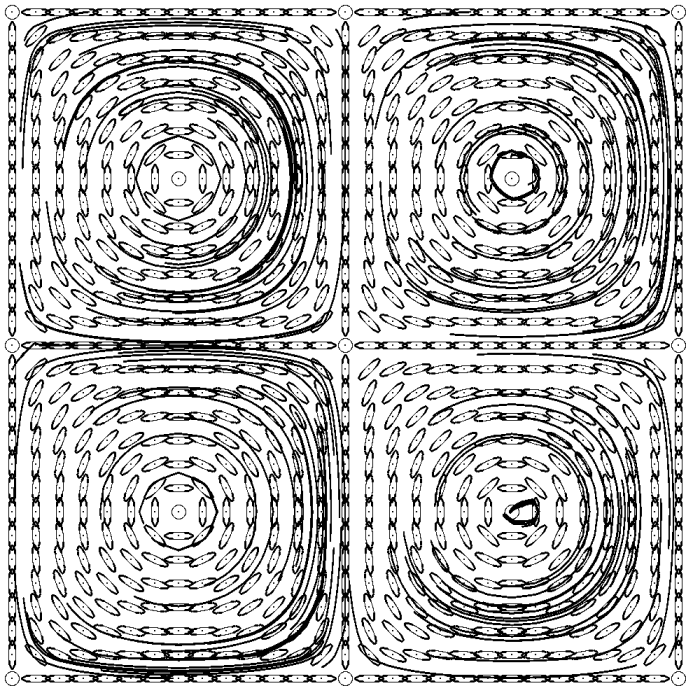
\includegraphics[height=0.7\textwidth]{img/gyre.png}
	{\scriptsize a)~Glyphs}
    \label{a)}
  \end{minipage}
  \begin{minipage}[t]{0.3\textwidth}
    \centering
    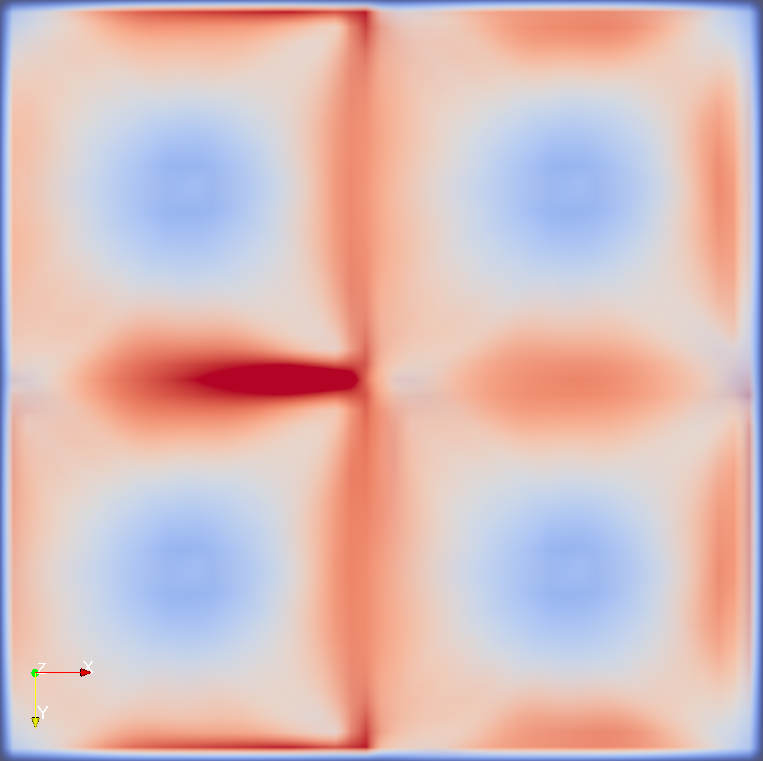
\includegraphics[height=0.7\textwidth]{gyre_ftle.PNG}
	{\scriptsize b)~LTG($0^\circ$)}
    \label{b)}
  \end{minipage}
  \begin{minipage}[t]{0.3\textwidth}
    \centering
    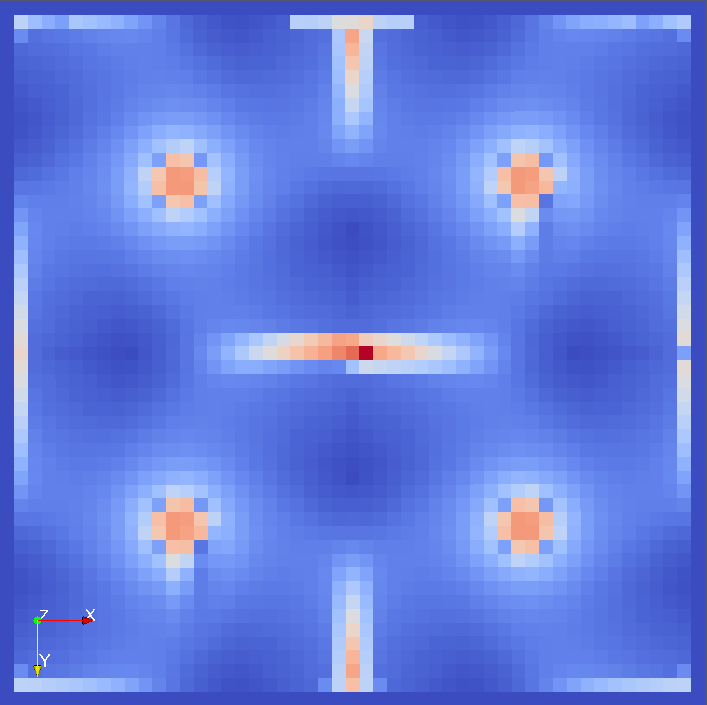
\includegraphics[height=0.7\textwidth]{gyre_ftle_org.PNG}
	{\scriptsize c)~}{\tiny T-FTLE: Hlawatsch's approach}
    \label{b)}
  \end{minipage}
\label{gyre-ftle}
\end{figure}
\bigskip
\begin{itemize}
	\item LTG is detecting ridges for diverging light distributions
	\item decreased response in gyre centers for circular overlap in difference image
\end{itemize}
} % END OF FRAME


\frame{
\frametitle{{Related Work - Asymmetric Tensor Field Visualization}}

\begin{itemize}
	\item dual eigenvectors\footnote[frame]{Zheng and Pang ''2d asymmetric tensor analysis", 2005}: use complex conjugate eigenvectors as co-visualization for the complex domain along with ordinary eigenvectors to represent the real domain
	\bigskip
	\item pseudo eigenvectors\footnote[frame]{Laramee et al. ''2d asymmetric tensor field topology", 2012}: extension for dual eigenvectors to a full set or graph
	\bigskip
	\item scalar measures: tensor magnitude\footnote[frame]{Lin et al. ''Asymmetric tensor field visualization for surfaces", 2011}, tensor mode\footnote[frame]{Palacios et al. ''Feature surfaces in symmetric tensor fields based on eigenvalue
manifold", 2015}, isotropy index\footnote[frame]{see footnote 12}
\end{itemize}

} % END OF FRAME


%\frame{
%\frametitle{{Light Transport Gradient - Scheme}}
%\begin{figure}[t]
%\centering
%  \begin{minipage}{0.6\textwidth}
%  \centering
%	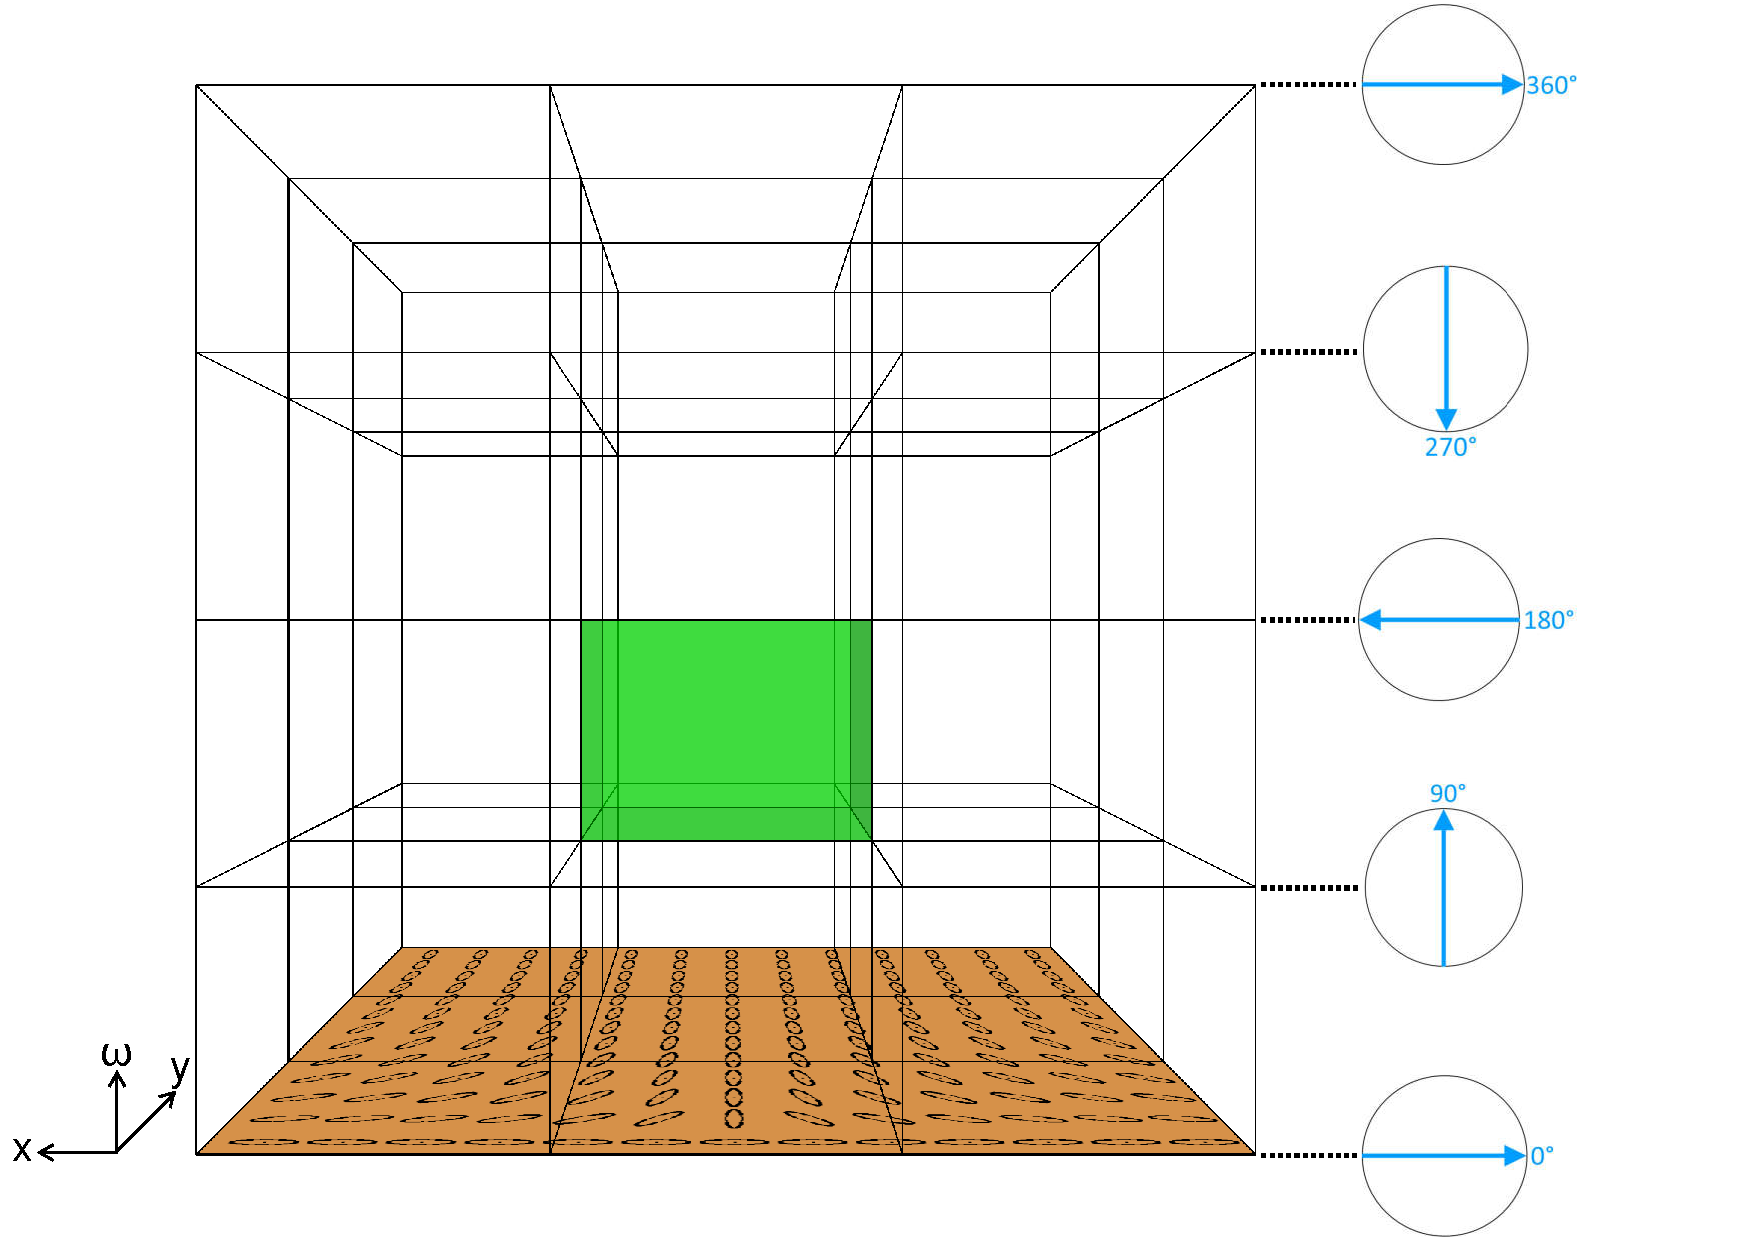
\includegraphics[height=0.7\textwidth]{skizze/addins/grids_one_base_edit.pdf}
%	\caption*{Light Transport Gradient - Domain of Light Distributions}
%	\end{minipage}
%\end{figure}
%
%} % END OF FRAME
%
%\frame{
%\frametitle{{Light Transport Gradient - Scheme}}
%\begin{figure}[t]
%\centering
%  \begin{minipage}{0.6\textwidth}
%  \centering
%	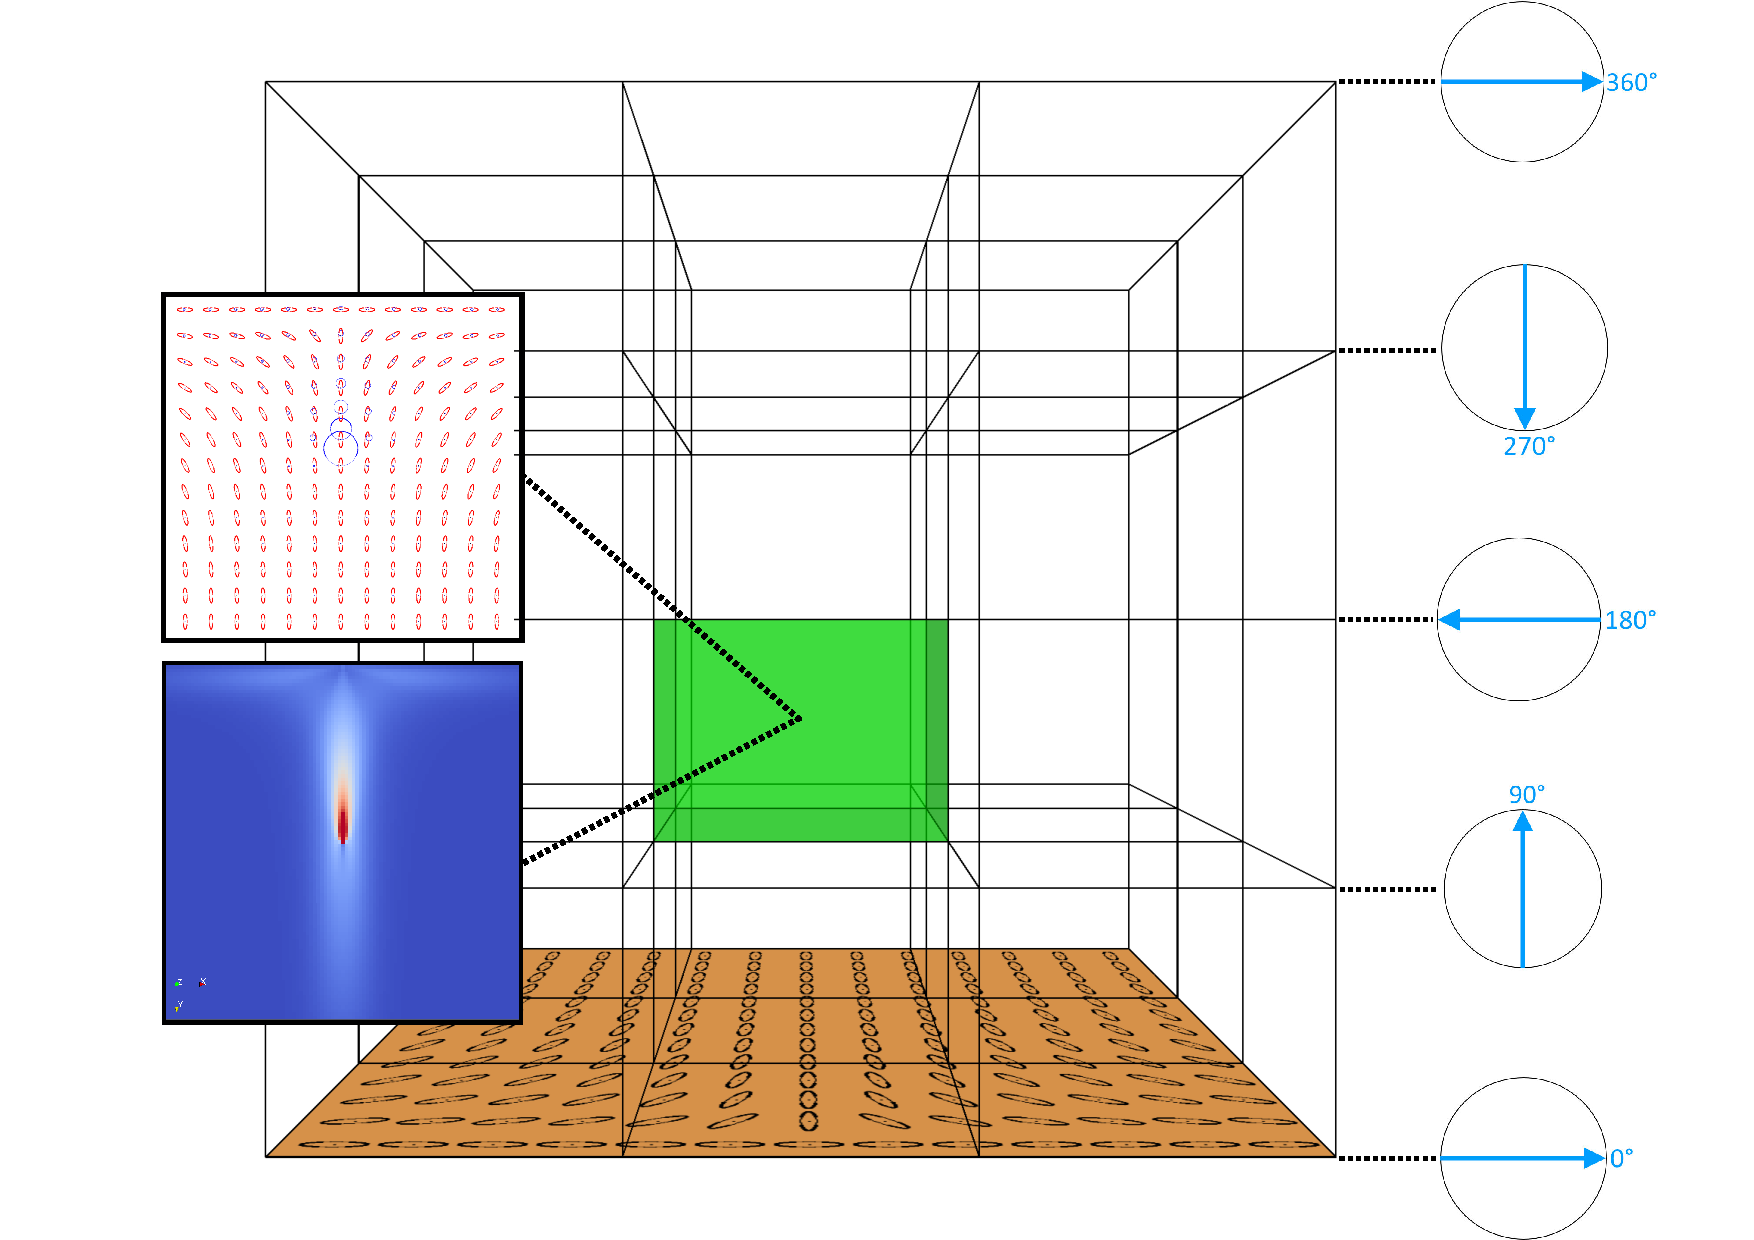
\includegraphics[height=0.7\textwidth]{skizze/addins/grids_one_edit.pdf}
%	\caption*{Light Transport Gradient - Domain of Light Distributions}
%	\end{minipage}
%\end{figure}
%
%} % END OF FRAME
%
%
%\frame{
%\frametitle{{Light Transport Gradient - Scheme}}
%\begin{figure}[t]
%\centering
%  \begin{minipage}{0.5\textwidth}
%  \centering
%	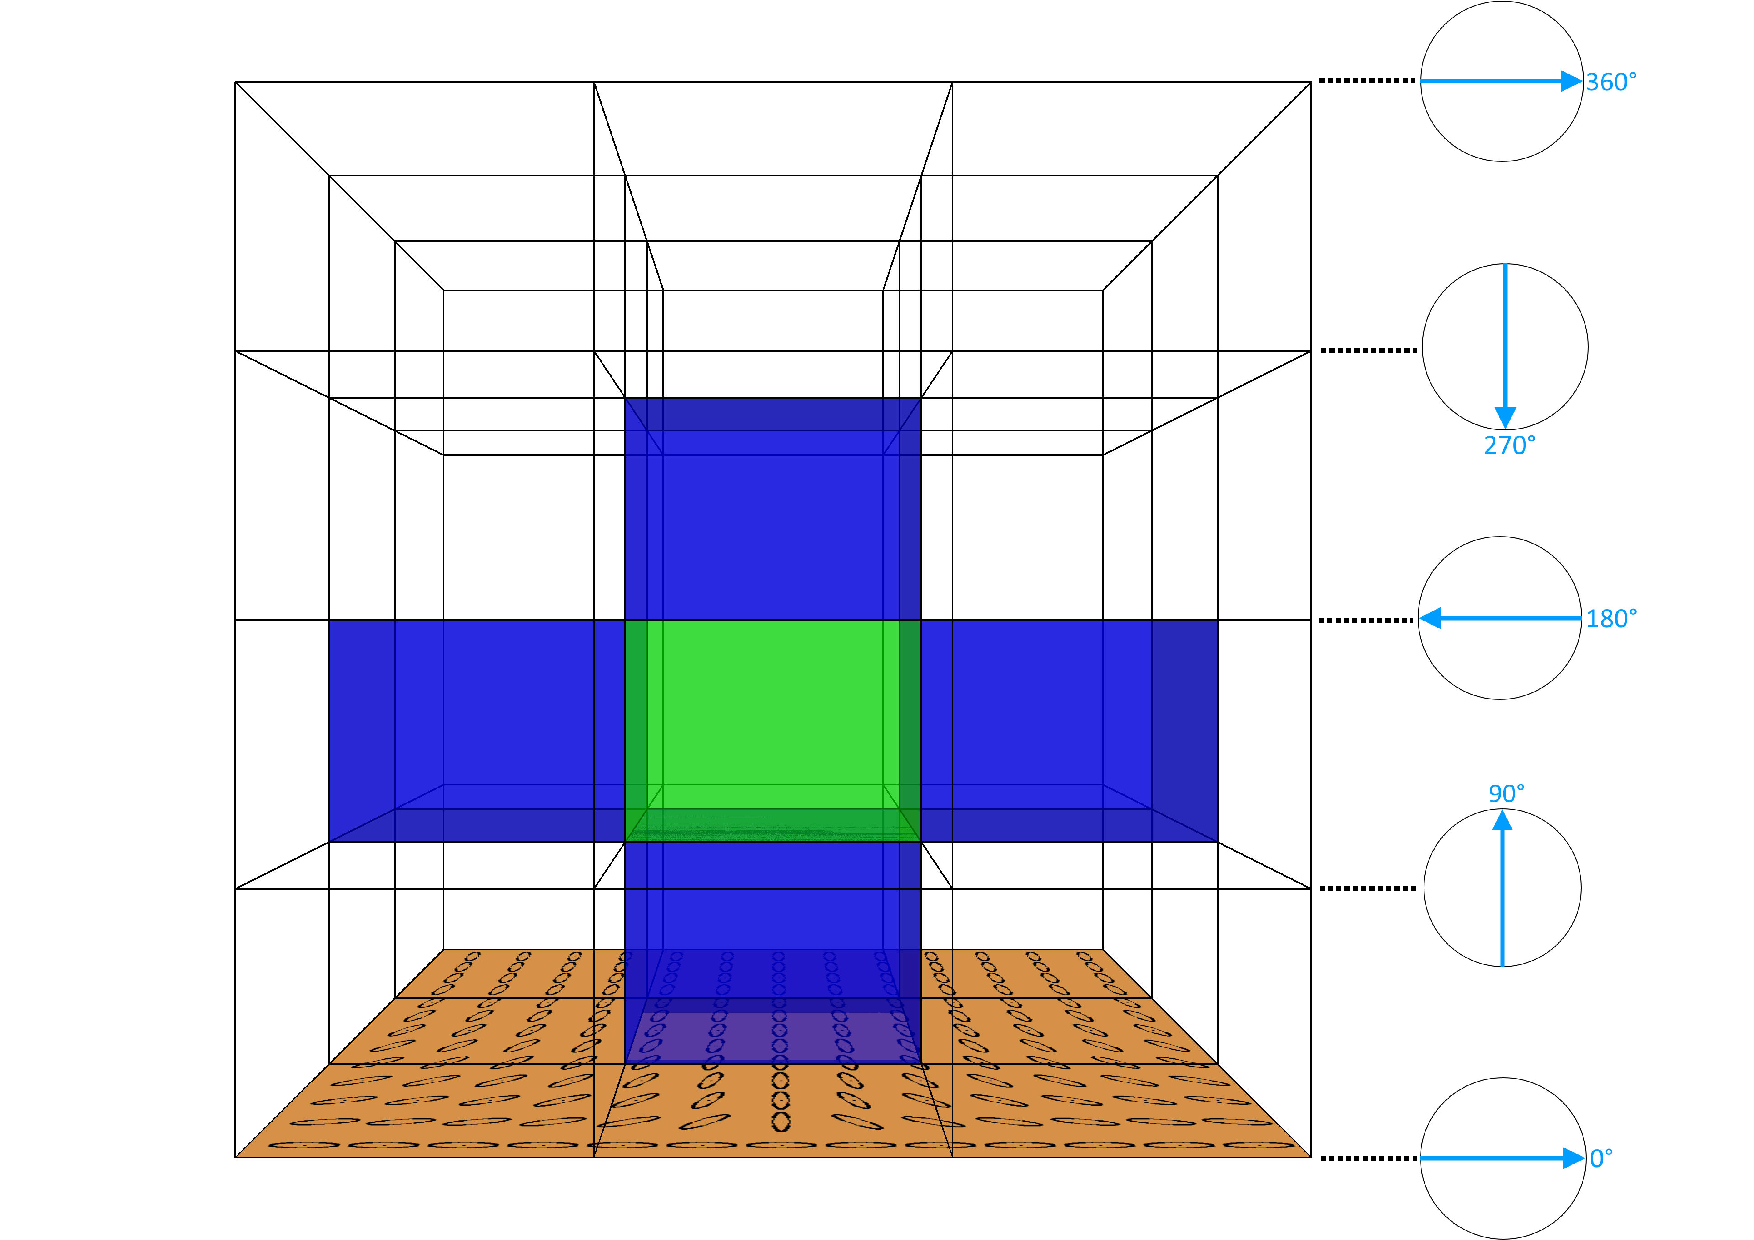
\includegraphics[height=0.85\textwidth]{skizze/addins/grid_two_base.pdf}
%	\caption*{Light Transport Gradient - Neighborhood}
%	\end{minipage}
%\end{figure}	
%
%} % END OF FRAME
%\frame{
%\frametitle{{Light Transport Gradient - Scheme}}
%\begin{figure}[t]
%\centering
%  \begin{minipage}{0.5\textwidth}
%  \centering
%	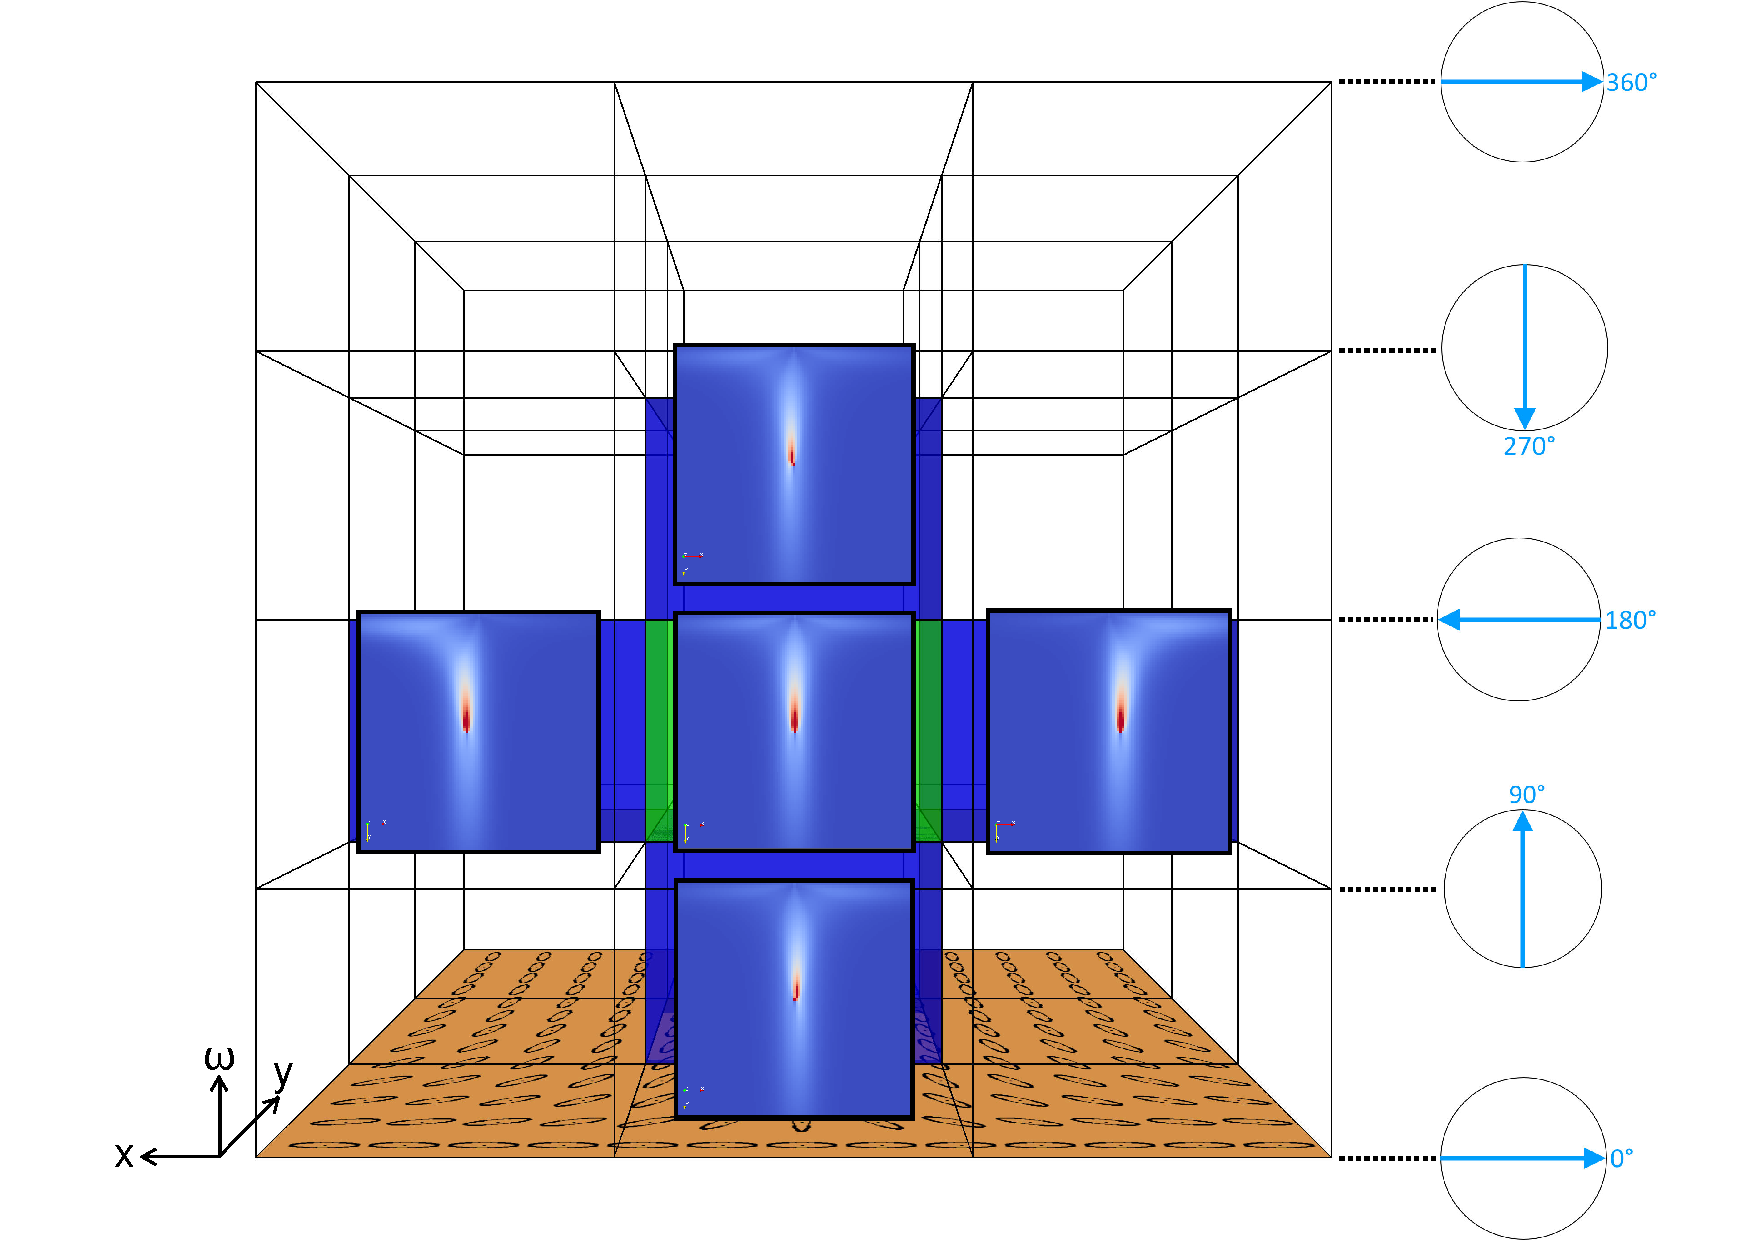
\includegraphics[height=0.85\textwidth]{skizze/addins/grids_two_edit.pdf}
%	\caption*{Light Transport Gradient - Neighborhood}
%	\end{minipage}
%\end{figure}
%
%} % END OF FRAME


%glyphs are used to represent the eigensystem, i.e., the anisotropy characteristics and/or tensor magnitude
%Volume non-directionally dependent


%%%%%%%%%%%%%%%%%%%%%%%%%%%%%%%%%%%%%%%%%%%%%%%%%%%%%%%%%%%%

% Alternative: put content in separate files
% Check the difference between including these files using \input{filename} and \include{filename} and see which one you like better
%\chapter{Einleitung}\label{intro}
%\input{introduction}
%
%\chapter{Voraussetzungen}\label{bg}
%\input{background}



\end{document}
